\chapter{Introduction to Software Development Methodologies}

\section{What is a Software Development Methodology?}

\textbf{Software development} is a complex process that requires careful planning and
execution. A software development methodology provides a structured approach to
managing this complexity, ensuring that projects are delivered on time, within
budget, and to the required quality. Understanding the purpose and different
types of methodologies is fundamental to becoming a successful software
engineer.

\subsection{What is a Software Development Methodology?}

A \textbf{software development methodology (SDM)} is a framework that is used
to structure, plan, and control the process of developing an information
system. It provides a systematic approach to building software, breaking down
the work into manageable phases. Think of it as a roadmap that guides the
development team from the initial concept to the final product.

\begin{figure}[ht]
  \centering
  
\includegraphics[width=0.8\textwidth]{images/software_development_lifecycle.png}
  \caption{Software Development Lifecycle}
  \label{fig:software_development_lifecycle}
\end{figure}

\subsection{Key Aspects of a Software Development Methodology}

To fully understand what an SDM is, let's break it down into key aspects:

\begin{conceptcard}{The Five Pillars of Software Development Methodologies}
  \begin{enumerate}
    \item \textbf{\faPlay\ Process}: An SDM defines the steps and activities involved in software development. These steps typically include requirements gathering, design, implementation, testing, deployment, and maintenance.

    \item \textbf{\faSitemap\ Structure}: It provides a structure for organizing the development process, specifying the order in which activities should be performed and the relationships between them.

    \item \textbf{\faBook\ Guidelines}: SDMs offer guidelines and best practices for performing each activity, ensuring consistency and quality throughout the development lifecycle.

    \item \textbf{\faTools\ Tools and Techniques}: SDMs often recommend or incorporate specific tools and techniques to support the development process, such as project management software, code repositories, and testing frameworks.

    \item \textbf{\faUsers\ Roles and Responsibilities}: A well-defined SDM specifies the roles and responsibilities of each team member, ensuring that everyone knows their part in the project.
  \end{enumerate}
\end{conceptcard}

% [IMAGE PLACEHOLDER: Infographic showing the 5 key aspects of SDM - Process, Structure, Guidelines, Tools & Techniques, and Roles & Responsibilities with icons and brief descriptions]

\subsection{Why Use a Software Development Methodology?}

There are several compelling reasons why software development teams use
methodologies:

\begin{highlightbox}{Key Benefits of Using Methodologies}
  \begin{itemize}
    \item \textbf{\faChartLine\ Improved Project Success Rates}: By providing a structured approach, SDMs increase the likelihood of delivering projects on time, within budget, and to the required quality.

    \item \textbf{\faComments\ Enhanced Communication and Collaboration}: SDMs facilitate communication and collaboration among team members, stakeholders, and clients.

    \item \textbf{\faShield*\ Better Risk Management}: SDMs help identify and mitigate potential risks early in the development process.

    \item \textbf{\faRocket\ Increased Efficiency and Productivity}: By streamlining the development process, SDMs improve efficiency and productivity.

    \item \textbf{\faStar\ Higher Quality Software}: SDMs promote the development of high-quality software that meets the needs of its users.

    \item \textbf{\faClock\ Predictability}: Methodologies bring predictability to the software development process. This is crucial for planning resources, setting realistic timelines, and managing expectations.
  \end{itemize}
\end{highlightbox}

Let's explore these benefits with examples:

\begin{examplebox}{Avoiding Scope Creep}
  Imagine a project to build an e-commerce website. Without a methodology, the client might continuously add new features during development (scope creep). This can lead to delays, increased costs, and a frustrated development team. A methodology like Agile, with its iterative approach and regular feedback loops, allows for managing changes in scope more effectively.
\end{examplebox}

\begin{examplebox}{Improved Communication}
  Consider a team working on a mobile application. Without a defined methodology, the designers, developers, and testers might have different understandings of the requirements. This can result in miscommunication, rework, and ultimately, a lower-quality product. An SDM promotes clear communication through defined processes and documentation.
\end{examplebox}

\begin{examplebox}{Risk Mitigation}
  Suppose a company is developing a new financial software. Without a proper methodology, they might not identify critical security vulnerabilities until late in the development cycle. This could lead to significant financial losses and reputational damage. Methodologies that incorporate risk assessment and mitigation strategies help prevent such issues.
\end{examplebox}

\subsection{Hypothetical Scenario: University Course Registration System}

Let's consider a hypothetical scenario. A university needs to develop a new
online course registration system. Without a software development methodology,
the project might encounter the following problems:

\begin{itemize}
  \item \textbf{Unclear Requirements}: The development team may not fully understand the needs of the students, faculty, and administrative staff.
  \item \textbf{Poor Communication}: Different stakeholders may have conflicting ideas about the system's functionality.
  \item \textbf{Lack of Coordination}: The development tasks may not be properly coordinated, leading to delays and errors.
  \item \textbf{Inadequate Testing}: The system may not be thoroughly tested before it is deployed, resulting in a buggy and unreliable product.
\end{itemize}

By adopting a software development methodology, such as Agile or Waterfall
(which we'll discuss later), the university can avoid these problems and ensure
the successful development of the course registration system.

\subsection{Types of Software Development Methodologies}

While we will delve into specific methodologies in subsequent lessons, it's
important to get an initial overview of some common types:

\begin{itemize}
  \item \textbf{Waterfall}: A linear, sequential approach where each phase must be completed before the next one begins.
  \item \textbf{Agile}: An iterative and incremental approach that emphasizes flexibility and collaboration. Scrum and Kanban are popular Agile frameworks.
  \item \textbf{Spiral}: A risk-driven approach that combines elements of Waterfall and iterative methodologies.
  \item \textbf{Rapid Application Development (RAD)}: An approach that emphasizes speed and rapid prototyping.
\end{itemize}

These methodologies are not mutually exclusive, and organizations often tailor
them to their specific needs.

\subsection{Waterfall Methodology: A Brief Introduction}

The Waterfall methodology is a traditional, sequential approach to software
development. It follows a strict, linear process, where each phase of the
development lifecycle must be completed before moving on to the next. These
phases typically include:

\begin{enumerate}
  \item \textbf{Requirements Gathering}: Defining the scope and objectives of the project.
  \item \textbf{Design}: Creating the system architecture and detailed design specifications.
  \item \textbf{Implementation}: Writing the code based on the design specifications.
  \item \textbf{Testing}: Verifying that the software meets the requirements and is free of defects.
  \item \textbf{Deployment}: Releasing the software to the users.
  \item \textbf{Maintenance}: Providing ongoing support and updates to the software.
\end{enumerate}

Waterfall is best suited for projects with well-defined requirements and a
stable scope. However, it can be inflexible and difficult to adapt to changes.
We'll explore this methodology in detail in the next lesson.

\subsection{Agile Methodology: A Brief Introduction}

Agile methodologies embrace iterative development, collaboration, and
adaptability. Unlike Waterfall, Agile projects are divided into small cycles
called sprints or iterations. Each sprint results in a working increment of the
software. Regular feedback and continuous improvement are key aspects of Agile.

Popular Agile frameworks include:

\begin{itemize}
  \item \textbf{Scrum}: A framework that defines specific roles, events, and artifacts to manage the development process.
  \item \textbf{Kanban}: A visual system for managing workflow and limiting work in progress.
\end{itemize}

Agile is well-suited for projects with evolving requirements and a need for
rapid feedback. We will have a dedicated lesson to dive deeper into Agile.

\subsection{Considerations for Choosing a Methodology}

Selecting the right software development methodology is a critical decision
that can significantly impact the success of a project. There is no
one-size-fits-all approach, and the best methodology will depend on several
factors:

\begin{itemize}
  \item \textbf{Project Size and Complexity}: For small, simple projects, a lightweight methodology like Kanban might be sufficient. For large, complex projects, a more structured methodology like Waterfall or a scaled Agile framework might be necessary.
  \item \textbf{Requirements Stability}: If the requirements are well-defined and unlikely to change, Waterfall might be a suitable option. If the requirements are evolving, an Agile methodology is generally preferred.
  \item \textbf{Team Size and Experience}: Agile methodologies require a highly collaborative and self-organizing team. If the team is small or lacks experience with Agile, a more structured methodology might be easier to implement.
  \item \textbf{Client Involvement}: Agile methodologies require a high degree of client involvement. If the client is not willing or able to actively participate in the development process, a different methodology might be more appropriate.
  \item \textbf{Organizational Culture}: The chosen methodology should align with the organization's culture and values.
\end{itemize}

\textbf{Example:}

A startup company developing a mobile app with limited resources and constantly
changing requirements might prefer an Agile methodology like Scrum. On the
other hand, a large government agency building a safety-critical system with
strict regulations might opt for a more structured methodology like Waterfall,
albeit adapted to incorporate feedback loops.

Choosing a methodology is not a one-time decision. As the project evolves, it
may be necessary to adapt or even change methodologies. The key is to be
flexible and choose the approach that best supports the project's goals.

\subsection{Real-World Application}

Consider two real-world scenarios:

\begin{enumerate}
  \item \textbf{Developing a New Mobile Banking App}: A bank decides to develop a new mobile banking application. Due to the rapidly evolving mobile technology landscape and the need to quickly respond to customer feedback, they choose an Agile methodology like Scrum. This allows them to release new features and updates frequently, based on user feedback and market trends.
  \item \textbf{Building an Air Traffic Control System}: A government agency is tasked with building a new air traffic control system. Due to the critical nature of the system and the strict safety regulations, they choose a Waterfall-based methodology with rigorous testing and documentation at each stage. This ensures that the system meets the highest standards of reliability and safety.
\end{enumerate}

These examples highlight the importance of selecting a methodology that is
appropriate for the specific project and its constraints.

\section{Waterfall Methodology}

The Waterfall methodology is a classic approach to software development,
characterized by its linear and sequential structure. Understanding it is
crucial because it forms the foundation upon which many other methodologies,
like Agile, build. Recognizing its strengths and weaknesses helps you
appreciate the evolution of software development practices and choose the most
appropriate methodology for a given project. Even though it is not as common as
Agile, the principles of Waterfall are still being used today in certain
fields, and is a good starting point for understanding the development process.

\subsection{Core Concepts of the Waterfall Methodology}

\begin{conceptcard}{What is the Waterfall Methodology?}
  The Waterfall methodology is a \textbf{sequential, non-iterative} design process. Each phase of the software development lifecycle (SDLC) must be \textbf{completed fully} before the next phase can begin. There is \textbf{no overlapping} in the waterfall model. Named ``Waterfall'' because the project flows steadily downwards through phases, much like a waterfall
\end{conceptcard}

\begin{figure}[ht]
  \centering
  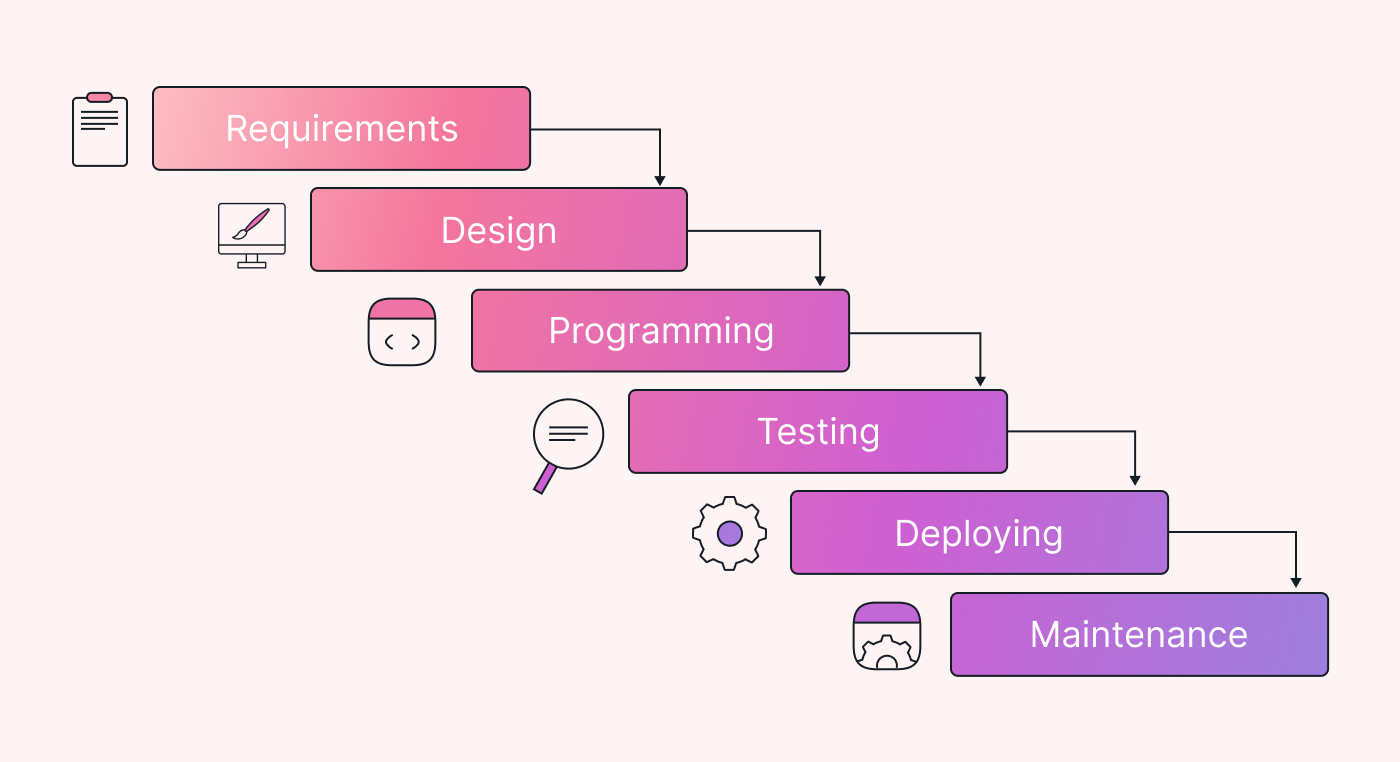
\includegraphics[width=0.8\textwidth]{images/waterfall_model.png}
  \caption{Waterfall Methodology Flow}
  \label{fig:waterfall_model}
\end{figure}

\subsection{Phases of the Waterfall Methodology}

The Waterfall methodology typically consists of the following phases:

\begin{conceptcard}{Waterfall Methodology Phases}
  \begin{enumerate}
    \item \textbf{Requirements Gathering and Analysis}: This is the initial phase where all possible requirements for the system to be designed are captured. These requirements are then documented in a requirement specification document.

          \begin{examplecard}{E-Commerce Website Requirements}
            Meeting with stakeholders to define the functionalities of an e-commerce website, documenting features like user accounts, product catalog, shopping cart, and payment gateway integration.
          \end{examplecard}

    \item \textbf{System Design}: The requirements from the first phase are used to design the system. This includes architectural design, database design, interface design, and more.

          \begin{examplecard}{Database and UI Design}
            Creating a database schema for the e-commerce website, outlining tables for products, users, orders, and categories. Defining the UI/UX for the website, including page layouts and navigation.
          \end{examplecard}

    \item \textbf{Implementation}: The actual coding of the system takes place in this phase. The design documents are translated into executable code.

          \begin{examplecard}{Frontend and Backend Development}
            Writing the HTML, CSS, and JavaScript code to create the front-end of the website. Implementing the back-end using a language like Python or Java to handle user authentication, product listings, and order processing.
          \end{examplecard}

    \item \textbf{Testing}: The system is tested to verify that it meets the requirements specified in the first phase. Different types of testing, such as unit testing, integration testing, and system testing, are performed.

          \begin{examplecard}{Comprehensive Testing Process}
            Testing user registration and login functionalities. Verifying that products can be added to the shopping cart and that the checkout process works correctly. Performing load testing to ensure the website can handle a large number of concurrent users.
          \end{examplecard}

    \item \textbf{Deployment}: The system is deployed to the production environment and made available to users.

          \begin{examplecard}{Production Deployment}
            Deploying the e-commerce website to a web server and configuring the domain name. Setting up a database server to store the website's data.
          \end{examplecard}

    \item \textbf{Maintenance}: After deployment, the system is maintained to fix any issues that arise, improve performance, and add new features.

          \begin{examplecard}{Ongoing System Maintenance}
            Monitoring the website for errors and performance issues. Fixing bugs reported by users. Adding new features, such as a customer review system or a loyalty program.
          \end{examplecard}
  \end{enumerate}
\end{conceptcard}

\subsection{Key Principles}

\begin{conceptcard}{Core Principles of Waterfall Methodology}
  \begin{itemize}
    \item \textbf{Sequential Progression}: Each phase must be completed before the next one begins. There is no going back to a previous phase once it is completed.

          \begin{examplecard}{Banking Application Development}
            In developing a banking application, the design phase cannot start until all the requirements, such as account management, transaction processing, and security features, are fully documented and approved.
          \end{examplecard}

    \item \textbf{Documentation}: Comprehensive documentation is created at each phase, serving as a blueprint for the subsequent phases.

          \begin{examplecard}{Hospital Management System Documentation}
            For a hospital management system, detailed documents would include requirement specifications, system design documents, test plans, user manuals, and maintenance logs.
          \end{examplecard}

    \item \textbf{Rigid Structure}: The Waterfall model follows a strict, inflexible structure. Changes to requirements are difficult and costly to implement once a phase is completed.

          \begin{examplecard}{Payroll System Regulation Change}
            If, halfway through the implementation of a payroll system, a new government regulation requires a change in tax calculation, it would be very difficult and expensive to incorporate that change without restarting the process.
          \end{examplecard}
  \end{itemize}
\end{conceptcard}

\subsection{Advantages and Disadvantages}

Understanding the pros and cons of Waterfall is essential for determining when
it is the right choice for a project.

\subsubsection{Advantages}

\begin{highlightbox}{Key Waterfall Advantages}
  \begin{itemize}
    \item \textbf{\faGraduationCap\ Simplicity}: The Waterfall model is easy to understand and implement. Its straightforward approach makes it suitable for projects with well-defined requirements.
          \begin{examplecard}{Data Conversion Tool}
            Building a simple data conversion tool where the input and output formats are known and unlikely to change demonstrates the simplicity advantage of Waterfall.
          \end{examplecard}
    \item \textbf{\faFile[regular]\ Clear Documentation}: Each phase produces detailed documentation, which makes it easier to understand the project's progress and maintain the system.
          \begin{examplecard}{Regulatory Compliance System}
            For a regulatory compliance system, comprehensive documentation ensures that all regulatory requirements are met and can be easily audited.
          \end{examplecard}
    \item \textbf{\faCalculator\ Predictable Costs}: Due to the well-defined nature of the model, it is easier to estimate project costs and timelines.
          \begin{examplecard}{Satellite Communication System}
            Developing a satellite communication system where the budget and schedule are predetermined based on contractual agreements showcases predictable costs.
          \end{examplecard}
    \item \textbf{\faLock\ Suitable for Stable Requirements}: The Waterfall model works well when the project requirements are fixed and unlikely to change during the development process.
          \begin{examplecard}{Automotive Embedded Systems}
            Developing embedded systems for automotive applications where the features are strictly defined by industry standards illustrates stable requirements.
          \end{examplecard}
  \end{itemize}
\end{highlightbox}

\subsubsection{Disadvantages}

\begin{warningbox}{Key Waterfall Limitations}
  \begin{itemize}
    \item \textbf{\faTimesCircle\ Inflexibility}: The Waterfall model is not well-suited for projects with evolving requirements. Changes are difficult and expensive to implement once a phase is completed.
          \begin{examplecard}{Social Media Platform}
            Creating a social media platform where user preferences and market trends can quickly change, requiring frequent updates and modifications demonstrates the inflexibility issue.
          \end{examplecard}
    \item \textbf{\faClock\ Delayed Testing}: Testing is done at the end of the development cycle, which means that any major issues may not be discovered until late in the process.
          \begin{examplecard}{ERP System Testing}
            For a large enterprise resource planning (ERP) system, finding critical bugs during system testing can result in significant delays and cost overruns.
          \end{examplecard}
    \item \textbf{\faEyeSlash\ Limited User Involvement}: Users are typically involved only in the initial requirements gathering phase, which can lead to a mismatch between the system and user needs.
          \begin{examplecard}{CRM Development Issues}
            Building a customer relationship management (CRM) system without continuous feedback from sales and marketing teams can result in a tool that doesn't effectively address their needs.
          \end{examplecard}
    \item \textbf{\faPause\ Risk of ``Analysis Paralysis''}: Teams can get bogged down in the initial phases (requirements gathering and design), leading to delays in starting the actual development.
  \end{itemize}
\end{warningbox}

\subsection{Practical Examples and Demonstrations}

To further illustrate the Waterfall methodology, let's explore a hypothetical
project and its application in different contexts.

\subsubsection{Example 1: Building a Simple Mobile App}

\begin{examplebox}{Water Intake Tracking App Development}
  \textbf{Scenario:} Imagine you are tasked with developing a basic mobile app for tracking daily water intake.

  \textbf{Requirements:}
  \begin{itemize}
    \item User can set a daily water intake goal.
    \item User can log the amount of water consumed throughout the day.
    \item The app displays a progress bar showing the percentage of the goal achieved.
    \item The app sends reminders to drink water at specified intervals.
  \end{itemize}

  \textbf{Using the Waterfall methodology:}
  \begin{enumerate}
    \item \textbf{Requirements Gathering and Analysis}: Document all the above requirements in detail, including specific data formats, reminder settings, and UI preferences.
    \item \textbf{System Design}: Design the app's architecture, including the database structure (if needed), UI layouts, and algorithms for calculating progress and scheduling reminders.
    \item \textbf{Implementation}: Write the code for the app, following the design specifications. This would involve coding the UI, implementing the logic for tracking water intake, and setting up the reminder system.
    \item \textbf{Testing}: Test the app thoroughly to ensure that all features work as expected, including setting goals, logging intake, displaying progress, and sending reminders.
    \item \textbf{Deployment}: Deploy the app to the app stores (e.g., Google Play Store, Apple App Store).
    \item \textbf{Maintenance}: Monitor the app for bugs and issues, and release updates as needed.
  \end{enumerate}
\end{examplebox}

\subsubsection{Example 2: Developing an Enterprise Resource Planning (ERP) System}

\begin{examplebox}{ERP System Development for Manufacturing Company}
  \textbf{Scenario:} A large manufacturing company needs to develop an ERP system to manage its operations, including inventory, supply chain, finance, and human resources.

  \textbf{Waterfall Implementation Process:}
  \begin{enumerate}
    \item \textbf{Requirements Gathering and Analysis}: Conduct extensive interviews with stakeholders from each department to gather detailed requirements. Document these requirements in a comprehensive specification document.
    \item \textbf{System Design}: Design the system architecture, including database schemas, module interfaces, and integration points. Create detailed design documents for each module.
    \item \textbf{Implementation}: Develop each module of the ERP system, following the design specifications. This would involve coding the inventory management module, supply chain module, finance module, and HR module.
    \item \textbf{Testing}: Conduct rigorous testing of each module and the entire system to ensure that it meets the requirements. This would include unit testing, integration testing, and system testing.
    \item \textbf{Deployment}: Deploy the ERP system to the company's servers and train employees on how to use it.
    \item \textbf{Maintenance}: Provide ongoing maintenance and support for the ERP system, including bug fixes, performance improvements, and new feature development.
  \end{enumerate}
\end{examplebox}

\subsubsection{Hypothetical Scenario: Government Infrastructure Project}

\begin{examplebox}{Bridge Construction Project}
  \textbf{Scenario:} Consider a government project to build a new bridge. The Waterfall methodology might be suitable here because the requirements are typically well-defined and unlikely to change significantly during the construction process.

  \textbf{Implementation Phases:}

  \begin{enumerate}
    \item \textbf{Requirements Gathering and Analysis}: Defining the bridge's specifications, such as length, width, load capacity, and materials.
    \item \textbf{System Design}: Creating detailed blueprints and engineering plans for the bridge.
    \item \textbf{Implementation}: Constructing the bridge according to the design plans.
    \item \textbf{Testing}: Inspecting the bridge to ensure it meets safety standards and load requirements.
    \item \textbf{Deployment}: Opening the bridge to public use.
    \item \textbf{Maintenance}: Performing regular maintenance and repairs to ensure the bridge remains safe and functional.
  \end{enumerate}
\end{examplebox}

\subsection{Exercises and Practice Activities}

To solidify your understanding of the Waterfall methodology, try the following
exercises:

\begin{enumerate}
  \item \textbf{Project Planning}: Choose a small project (e.g., developing a simple to-do list application) and create a detailed project plan using the Waterfall methodology. Outline the tasks, timelines, and deliverables for each phase.
  \item \textbf{Requirements Analysis}: Imagine you are developing a library management system. Write a detailed requirements specification document outlining the features and functionalities of the system.
  \item \textbf{Design Documentation}: Based on the requirements for the library management system, create a system design document that includes database schemas, UI layouts, and module interfaces.
  \item \textbf{Case Study Analysis}: Research a real-world project that used the Waterfall methodology and analyze its success or failure. Identify the factors that contributed to the outcome.
\end{enumerate}

\subsection{Real-World Application}

\begin{itemize}
  \item \textbf{Construction Projects}: As illustrated in the hypothetical government infrastructure project, the construction industry often uses Waterfall due to the well-defined requirements and structured approach.
  \item \textbf{Medical Device Development}: Medical device development often follows a Waterfall approach due to the strict regulatory requirements and need for comprehensive documentation.
  \item \textbf{Large-Scale Enterprise Systems}: Some large organizations with stable requirements may still use Waterfall for developing enterprise systems, such as ERP or CRM systems.
\end{itemize}

% \subsection{Key Takeaways}

% In conclusion, the Waterfall methodology provides a structured and sequential
% approach to software development that is best suited for projects with
% well-defined requirements and stable environments. While it may not be as
% flexible as Agile methodologies, it offers clear documentation, predictable
% costs, and ease of understanding. Understanding its strengths and weaknesses is
% crucial for choosing the right methodology for your project.

% \textbf{Key Points to Remember:}

% \begin{itemize}
%   \item The Waterfall methodology follows a linear, sequential approach with distinct
%         phases that must be completed before moving to the next.
%   \item It emphasizes comprehensive documentation and thorough planning upfront.
%   \item Best suited for projects with stable, well-defined requirements and minimal
%         expected changes.
%   \item Provides predictable timelines and costs, making it suitable for contractual
%         agreements.
%   \item Major disadvantages include inflexibility to change, delayed testing, and
%         limited user involvement throughout the process.
%   \item Still relevant today in industries requiring strict documentation and
%         regulatory compliance, such as healthcare, aerospace, and government projects.
%   \item Understanding Waterfall provides a foundation for appreciating the evolution to
%         more flexible methodologies like Agile.
% \end{itemize}

\section{Agile Methodology}

Agile methodology represents a significant shift from traditional, linear
approaches like the Waterfall model. Its emphasis on iterative development,
collaboration, and flexibility allows teams to respond effectively to changing
requirements and deliver value incrementally. Understanding Agile's core
principles and practices is crucial for any software engineer looking to thrive
in today's dynamic development landscape. This lesson will delve into the heart
of Agile, exploring its key concepts, benefits, and how it contrasts with more
rigid methodologies.

\begin{figure}[ht]
  \centering
  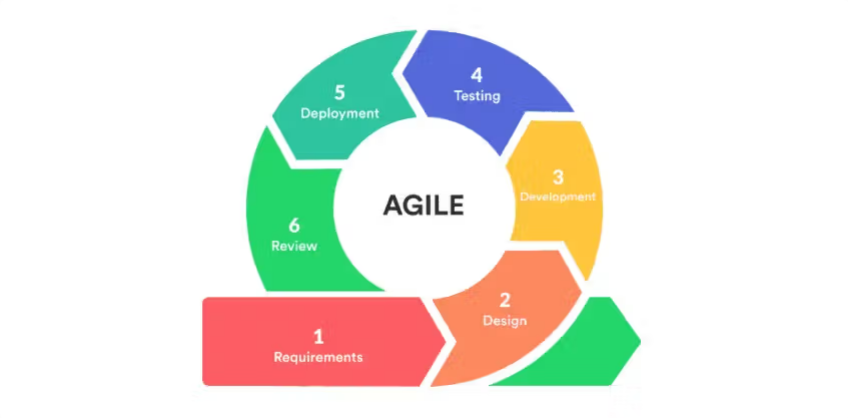
\includegraphics[width=0.8\textwidth]{images/agile_methodology.png}
  \caption{The Agile Methodology}
  \label{fig:agile_methodology}
\end{figure}

\subsection{Core Principles of Agile Methodology}

\begin{conceptcard}{The Agile Manifesto Core Values}
  \faUsers\ \textbf{Individuals and interactions} over processes and tools

  \faCode\ \textbf{Working software} over comprehensive documentation

  \faHandshake\ \textbf{Customer collaboration} over contract negotiation

  \faSync\ \textbf{Responding to change} over following a plan
\end{conceptcard}

The Agile Manifesto, published in 2001, outlines the four core values and
twelve principles that underpin the Agile methodology. These principles serve
as a guide for Agile teams and influence how they approach software
development. Let's break down these key concepts:

% [IMAGE PLACEHOLDER: The Agile Manifesto diagram showing the four core values with visual emphasis on "over" comparisons]


\begin{conceptcard}{Agile Manifesto Values}
  \begin{enumerate}
    \item \textbf{Individuals and interactions over processes and tools}: Agile prioritizes direct communication and collaboration among team members over strict adherence to processes and reliance on specific tools. This doesn't mean processes and tools are unimportant, but rather that they should support, not hinder, human interaction.

          \begin{examplecard}{Daily Stand-up vs Complex Tracking}
            Instead of relying solely on a complex issue tracking system, an Agile team might prefer daily stand-up meetings to discuss progress and roadblocks, fostering quicker problem-solving and knowledge sharing.
          \end{examplecard}

    \item \textbf{Working software over comprehensive documentation}: Agile emphasizes delivering functional software as the primary measure of progress, rather than spending excessive time on detailed documentation that may become outdated quickly. While documentation is still important, it should be concise, relevant, and focused on supporting the software.

          \begin{examplecard}{Functional Prototype vs Lengthy Documents}
            In Agile, creating a functional prototype that demonstrates core features and can be tested by users is valued more than writing a lengthy requirements document that may not accurately reflect the user's needs.
          \end{examplecard}

    \item \textbf{Customer collaboration over contract negotiation}: Agile emphasizes continuous collaboration with the customer throughout the development process to ensure that the software meets their evolving needs. This involves actively seeking feedback, incorporating suggestions, and adapting the software accordingly.

          \begin{examplecard}{Regular Demos and Feedback}
            An Agile team regularly demonstrates working software to the customer and solicits feedback. They incorporate this feedback into subsequent iterations, ensuring that the final product aligns closely with the customer's expectations.
          \end{examplecard}

    \item \textbf{Responding to change over following a plan}: Agile recognizes that change is inevitable in software development and embraces the ability to adapt to changing requirements throughout the project lifecycle. This involves being flexible, responsive, and willing to adjust plans as needed.

          \begin{examplecard}{Adaptive Design Approach}
            An Agile team discovers a critical flaw in their initial design during testing. Instead of sticking to the original plan, they quickly adapt their design to address the flaw, minimizing its impact on the project schedule.
          \end{examplecard}
  \end{enumerate}
\end{conceptcard}

\subsection{Iterative and Incremental Development}

At the heart of Agile lies iterative and incremental development. These two
concepts are closely related but distinct:

\begin{conceptcard}{Iterative and Incremental Development}
  \begin{itemize}
    \item \textbf{Iterative Development}: This involves breaking down the project into smaller cycles called iterations (often called Sprints in Scrum). Each iteration involves planning, designing, implementing, testing, and evaluating a portion of the software. The results of each iteration are then used to refine the requirements and design for subsequent iterations.

          \begin{examplecard}{E-Commerce Website Development Iterations}
            An e-commerce website is developed in iterations. The first iteration might focus on implementing the basic product catalog and browsing functionality. The second iteration might add user accounts and a shopping cart. The third iteration might implement payment processing and order management.
          \end{examplecard}

          \textbf{Benefits}: Early feedback, reduced risk, continuous improvement.

    \item \textbf{Incremental Development}: This involves delivering small, functional pieces of the software in each iteration. Each increment adds new functionality to the existing software, gradually building up the complete product.

          \begin{examplecard}{Functional Increments Delivery}
            Each iteration of the e-commerce website delivers a fully functional increment of the software. The first increment allows users to browse the product catalog. The second increment allows users to add products to a shopping cart. The third increment allows users to complete the checkout process.
          \end{examplecard}

          \textbf{Benefits}: Early value delivery, reduced complexity, easier testing.
  \end{itemize}
\end{conceptcard}

The combination of iterative and incremental development allows Agile teams to
deliver value early and often, respond quickly to change, and continuously
improve the software based on feedback.

\subsection{Benefits of Agile Methodology}

Agile offers numerous benefits over traditional methodologies, including:

\begin{itemize}
  \item \textbf{Increased Customer Satisfaction}: Continuous customer collaboration and early delivery of working software lead to higher customer satisfaction. Customers have the opportunity to provide feedback throughout the development process, ensuring that the final product meets their needs.
        \begin{examplecard}{Customer Feedback Integration}
          A customer sees a demo of the software after each iteration and provides feedback. The team incorporates this feedback into the next iteration, ensuring that the software evolves to meet the customer's changing needs.
        \end{examplecard}

  \item \textbf{Improved Product Quality}: Iterative development and continuous testing help to identify and fix defects early in the development process, leading to improved product quality.

        \begin{examplecard}{Automated Testing Benefits}
          Automated tests are run after each iteration to ensure that the software meets the required quality standards. Defects are fixed immediately, preventing them from accumulating and causing more serious problems later in the project.
        \end{examplecard}

  \item \textbf{Increased Project Visibility}: Agile methodologies emphasize transparency and communication, providing stakeholders with increased visibility into the project's progress.

        \begin{examplecard}{Project Transparency}
          Daily stand-up meetings, sprint reviews, and burndown charts provide stakeholders with a clear picture of the project's status and any potential risks.
        \end{examplecard}

  \item \textbf{Reduced Risk}: Early and frequent delivery of working software reduces the risk of delivering a product that does not meet the customer's needs or that is not of sufficient quality.

        \begin{examplecard}{Early Risk Management}
          The team identifies and addresses potential risks early in the project, preventing them from escalating into major problems. Regular demos allow the customer to validate the software and identify any areas that need improvement.
        \end{examplecard}

  \item \textbf{Increased Team Morale}: Agile methodologies empower teams to make decisions and take ownership of their work, leading to increased team morale and productivity.

        \begin{examplecard}{Self-Organizing Teams}
          Self-organizing teams are empowered to make decisions about how to best implement the software. This autonomy leads to increased team morale and a greater sense of ownership.
        \end{examplecard}

\end{itemize}

\subsection{Comparing Agile to Waterfall}

As introduced in the previous lesson, the Waterfall methodology follows a
sequential, linear approach. Agile, in contrast, embraces iteration and
flexibility. Here's a table highlighting the key differences:

\begin{table}[!h]
  \centering
  \begin{tabular}{p{4cm}|p{5cm}|p{5cm}}
    \hline
    \textbf{Feature}     & \textbf{Waterfall}                                                  & \textbf{Agile}                                  \\
    \hline
    Approach             & Sequential, linear                                                  & Iterative, incremental                          \\
    \hline
    Requirements         & Defined upfront                                                     & Evolving, adaptable                             \\
    \hline
    Customer Involvement & Limited after initial requirements gathering                        & Continuous throughout the development process   \\
    \hline
    Change Management    & Difficult and costly                                                & Embraces change                                 \\
    \hline
    Risk Management      & High risk of delivering a product that does not meet customer needs & Reduced risk due to early and frequent feedback \\
    \hline
    Documentation        & Comprehensive                                                       & Concise and relevant                            \\
    \hline
  \end{tabular}
  \caption{Comparison of Waterfall and Agile Methodologies}
  \label{tab:waterfall_vs_agile}
\end{table}

% [IMAGE PLACEHOLDER: Side-by-side visual comparison of Waterfall vs Agile showing sequential vs iterative approaches with icons and timelines]

\textbf{Hypothetical Scenario:}

Imagine developing a mobile app for ordering food.

\begin{itemize}
  \item \textbf{Waterfall Approach}: All requirements (features, design, functionality) are defined upfront. The team then proceeds through design, implementation, testing, and deployment in a linear fashion. If the market trends change during development (e.g., users start demanding new features like real-time order tracking), adapting to these changes becomes difficult and costly.

  \item \textbf{Agile Approach}: The team starts with a basic version of the app that allows users to browse menus and place orders. After each iteration (e.g., a two-week sprint), they add new features based on user feedback and market trends (e.g., real-time order tracking, loyalty programs). This allows them to adapt to changing requirements and deliver a product that meets the evolving needs of the users.
\end{itemize}

\subsection{Exercises}

\begin{enumerate}
  \item \textbf{Agile Values Identification}: For the following scenarios, identify which Agile value is being exemplified (Individuals and interactions, Working software, Customer collaboration, Responding to change):
        \begin{itemize}
          \item A developer pair-programs with a tester to resolve a critical bug quickly.
          \item A team decides to refactor a complex module to improve its maintainability.
          \item A product owner regularly seeks feedback from users on new features.
          \item A team releases a minimal viable product (MVP) to gather early user feedback.
        \end{itemize}

  \item \textbf{Waterfall vs. Agile}: Consider a project to develop a new accounting software for a small business. Discuss the advantages and disadvantages of using Waterfall versus Agile for this project. Consider factors like the business's familiarity with software development, the stability of requirements, and the need for rapid delivery.

  \item \textbf{Iterative vs. Incremental}: Explain the difference between iterative and incremental development in your own words. Provide an example of a project and how it could be developed using both approaches.
\end{enumerate}

\subsection{Real-World Application}

Consider Spotify, the popular music streaming service. Spotify likely utilizes
Agile methodologies to continuously improve its platform. New features, such as
collaborative playlists, enhanced audio quality, or personalized
recommendations, are likely developed and released in iterations. User feedback
is continuously gathered and incorporated into future iterations, ensuring that
the platform remains relevant and meets the evolving needs of its users. The
company's ability to rapidly deploy new features and adapt to changing user
preferences is a testament to the power of Agile methodologies.

Another real-world example is Tesla. Their software development teams use Agile
to deploy new features to their vehicles over the air. This iterative approach
allows them to quickly respond to customer feedback and continuously improve
the driving experience.

Agile methodology provides a framework for software development that emphasizes
collaboration, flexibility, and continuous improvement. By embracing its core
principles and practices, teams can deliver high-quality software that meets
the evolving needs of their customers. In the next lesson, we will focus on one
of the most popular Agile frameworks: Scrum, and the roles, artifacts, and
events that are used in this framework.

\section{Scrum Framework: Roles, Events, and Artifacts}

Scrum is a lightweight framework that helps teams work together. It encourages
teams to learn through experiences, self-organize while solving a problem, and
reflect on their wins and losses to continuously improve. Unlike Waterfall,
which is sequential and rigid, Scrum embraces change and allows for iterative
development. In this lesson, we'll dive into the core components of Scrum: its
roles, events, and artifacts. Understanding these elements is crucial for
effectively implementing Scrum in software development and other projects.

% [IMAGE PLACEHOLDER: Scrum framework overview diagram showing the three pillars (Roles, Events, Artifacts) with interconnected elements]

\subsection{Scrum Roles}

In Scrum, there are three distinct roles, each with specific responsibilities
and accountabilities. These roles are designed to promote self-organization,
collaboration, and efficiency within the Scrum team.

% [IMAGE PLACEHOLDER: Scrum roles diagram showing Product Owner, Scrum Master, and Development Team with their key responsibilities listed]

\subsubsection{Product Owner}

The Product Owner is responsible for maximizing the value of the product
resulting from the work of the Development Team. They are the voice of the
customer and stakeholders, and they manage the Product Backlog to ensure it
reflects the desired features, enhancements, and fixes.

\textbf{Responsibilities of the Product Owner:}

\begin{itemize}
  \item \textbf{Defining the Product Backlog}: The Product Owner creates and maintains the Product Backlog, which is an ordered list of everything that might be needed in the product.
  \item \textbf{Prioritizing the Product Backlog}: They are responsible for ordering the items in the Product Backlog based on value, risk, priority, and dependencies. This ensures the Development Team works on the most important items first.
  \item \textbf{Ensuring Transparency}: The Product Owner makes sure the Product Backlog is visible, transparent, and clear to everyone, and that the Development Team understands the items to the level needed.
  \item \textbf{Stakeholder Management}: They gather feedback from stakeholders, understand their needs, and incorporate them into the Product Backlog.
  \item \textbf{Accepting or Rejecting Work Results}: At the end of each Sprint, the Product Owner reviews the work completed by the Development Team and decides whether to accept or reject it based on the Definition of Done (which we'll discuss later).
\end{itemize}

\begin{examplecard}{Study Group App Product Owner Scenario}
  Imagine a college project to develop a mobile application for students to find study groups. The Product Owner, Sarah, would gather requirements from students (the users) about the app's features: creating profiles, searching for groups, scheduling meetings, etc. She would then create a Product Backlog listing these features, prioritizing them based on which features would provide the most value to the students first. For instance, the ability to search for study groups might be prioritized higher than creating detailed profiles.
\end{examplecard}

\subsubsection{Scrum Master}

The Scrum Master is a servant-leader for the Scrum Team. They are responsible
for ensuring that Scrum is understood and enacted. They do this by ensuring
that the Scrum Team adheres to Scrum theory, practices, and rules. The Scrum
Master helps those outside the Scrum Team understand which of their
interactions with the Scrum Team are helpful and which aren't. The Scrum Master
removes impediments that hinder the Development Team's progress.

\textbf{Responsibilities of the Scrum Master:}

\begin{itemize}
  \item \textbf{Facilitating Scrum Events}: The Scrum Master facilitates Scrum events (Sprint Planning, Daily Scrum, Sprint Review, and Sprint Retrospective) to ensure they are productive and within the timebox.
  \item \textbf{Coaching the Scrum Team}: They coach the Development Team in self-organization and cross-functionality.
  \item \textbf{Removing Impediments}: The Scrum Master identifies and removes obstacles that are hindering the Development Team's progress. This could be anything from technical issues to organizational roadblocks.
  \item \textbf{Protecting the Scrum Team}: They shield the Development Team from external interference to ensure they can focus on their work.
  \item \textbf{Coaching the Product Owner}: The Scrum Master also coaches the Product Owner in Product Backlog management and maximizing the value of the product.
  \item \textbf{Promoting Scrum}: They promote understanding of Scrum within the organization.
\end{itemize}

\textbf{Example Scenario:}

Continuing with the college project, the Scrum Master, David, would ensure the
team understands Scrum principles. If the Development Team is consistently late
delivering features because they are waiting on feedback from the Product
Owner, David would work with Sarah (the Product Owner) to improve communication
and ensure timely feedback. He would also facilitate the Daily Scrum meetings,
ensuring they are concise and focused.

\subsubsection{Development Team}

The Development Team consists of professionals who do the work of delivering a
potentially releasable Increment of "Done" product at the end of each Sprint.
The Development Team is self-organizing and cross-functional.

\textbf{Characteristics of the Development Team:}

\begin{itemize}
  \item \textbf{Self-Organizing}: No one (not even the Scrum Master) tells the Development Team how to turn Product Backlog into Increments of potentially releasable product.
  \item \textbf{Cross-Functional}: The Development Team possesses all the skills necessary to create a product Increment.
  \item \textbf{Accountable}: The Development Team is accountable for creating a plan for the Sprint (Sprint Backlog), instilling quality by adhering to a Definition of Done, adapting their plan each day toward the Sprint Goal, and holding themselves accountable as professionals.
  \item \textbf{Team Size}: Optimal Development Teams are small enough to remain nimble and large enough to complete significant work within a Sprint. Usually, the ideal size is 3-9 members. Smaller teams may encounter skill constraints, and larger teams can generate too much complexity to manage empirically.
\end{itemize}

\textbf{Example Scenario:}

In the college project, the Development Team might consist of students with
skills in mobile app development, UI/UX design, and testing. They work together
to design, build, and test the app features defined in the Product Backlog.
They decide how to break down the work and assign tasks among themselves. They
are also responsible for ensuring the quality of the app by adhering to a
Definition of Done, which might include writing unit tests and conducting user
testing.

\begin{examplecard}{E-Commerce Platform Development}
  Consider a software company developing a new e-commerce platform:
  \begin{itemize}
    \item \textbf{Product Owner}: Responsible for defining the features of the platform, prioritizing them based on customer needs and business value, and managing the Product Backlog.
    \item \textbf{Scrum Master}: Ensures the Scrum team follows Scrum principles, facilitates Scrum events, removes impediments, and coaches the team.
    \item \textbf{Development Team}: Designs, develops, tests, and delivers the features of the e-commerce platform.
  \end{itemize}
\end{examplecard}

\begin{examplecard}{Marketing Agency Campaign}
  A marketing agency managing a client's advertising campaign:
  \begin{itemize}
    \item \textbf{Product Owner}: Defines the goals of the campaign, prioritizes marketing activities, and manages the campaign backlog.
    \item \textbf{Scrum Master}: Facilitates the campaign planning, removes obstacles, and ensures the team adheres to the Scrum framework.
    \item \textbf{Development Team}: Creates advertising content, manages ad spend, and analyzes campaign performance.
  \end{itemize}
\end{examplecard}

\begin{examplecard}{Charity Event Organization}
  Imagine a group of friends organizing a charity event:
  \begin{itemize}
    \item \textbf{Product Owner}: Decides on the type of event, sets fundraising goals, and prioritizes tasks like securing a venue, sponsors, and entertainment.
    \item \textbf{Scrum Master}: Helps the group follow a structured process, facilitates planning meetings, and removes obstacles such as difficulty contacting potential sponsors.
    \item \textbf{Development Team}: Handles various tasks like marketing, logistics, volunteer coordination, and fundraising.
  \end{itemize}
\end{examplecard}

\subsection{Scrum Events}

Scrum events are time-boxed meetings that provide structure and opportunities
for inspection and adaptation. These events are designed to facilitate
communication, collaboration, and progress toward the Sprint Goal.

% [IMAGE PLACEHOLDER: Scrum Events timeline diagram showing Sprint Planning → Daily Scrum → Sprint Review → Sprint Retrospective in a cyclical pattern within a Sprint timeframe]

\subsubsection{Sprint}

The Sprint is the heart of Scrum. It is a time-boxed period (typically 1-4
weeks) during which the Development Team works to complete a set of Product
Backlog items and deliver a potentially releasable Increment of the product.

\textbf{Key Characteristics of a Sprint:}

\begin{itemize}
  \item \textbf{Fixed Duration}: Sprints have a fixed start and end date. Once a Sprint begins, its duration should not be changed.
  \item \textbf{Consistent Cadence}: Sprints should be of consistent length to establish a predictable rhythm for the Development Team.
  \item \textbf{Sprint Goal}: Each Sprint has a Sprint Goal, which is an objective that the Development Team will achieve during the Sprint. The Sprint Goal provides focus and direction for the Sprint.
  \item \textbf{No Changes to Goal}: While the Development Team can make some adjustments to the Sprint Backlog, the Sprint Goal remains fixed.
\end{itemize}

\begin{examplecard}{College Project Sprint Example}
  In the college project, a Sprint might be two weeks long. The Sprint Goal could be to ``Develop a functional prototype of the study group search feature.'' During this Sprint, the Development Team would focus solely on designing, building, and testing this feature.
\end{examplecard}

\subsubsection{Sprint Planning}

Sprint Planning is an event that occurs at the beginning of each Sprint. During
Sprint Planning, the Scrum Team collaborates to plan the work that will be
performed during the Sprint.

\textbf{Key Activities in Sprint Planning:}

\begin{itemize}
  \item \textbf{Selecting Product Backlog Items}: The Product Owner presents the prioritized Product Backlog items, and the Development Team selects the items they can commit to completing during the Sprint.
  \item \textbf{Creating the Sprint Backlog}: The Development Team creates a Sprint Backlog, which is a detailed plan for how they will complete the selected Product Backlog items. This includes breaking down the items into smaller tasks and estimating the effort required for each task.
  \item \textbf{Defining the Sprint Goal}: The Scrum Team defines the Sprint Goal, which is a short description of what the Sprint will achieve.
\end{itemize}

\begin{examplecard}{Sprint Planning Session}
  Before starting a two-week Sprint, Sarah (Product Owner) presents the top items from the Product Backlog related to study group search. The Development Team estimates the effort required for each item and commits to completing specific tasks like ``Implement search algorithm,'' ``Design search results display,'' and ``Write unit tests for search functionality.'' They then define the Sprint Goal as ``Develop a functional prototype of the study group search feature.''
\end{examplecard}

\subsubsection{Daily Scrum}

The Daily Scrum is a short (typically 15-minute) meeting held each day of the
Sprint. It is a time for the Development Team to synchronize their activities
and create a plan for the next 24 hours.

\textbf{Key Aspects of the Daily Scrum:}

\begin{itemize}
  \item \textbf{Time-boxed}: The Daily Scrum is strictly time-boxed to 15 minutes to keep it focused and efficient.
  \item \textbf{Development Team Focus}: The Daily Scrum is primarily for the Development Team. The Product Owner and Scrum Master may attend, but they should not dominate the discussion.
  \item \textbf{Three Questions}: Traditionally, each Development Team member answers three questions:
        \begin{itemize}
          \item What did I do yesterday that helped the Development Team meet the Sprint Goal?
          \item What will I do today to help the Development Team meet the Sprint Goal?
          \item Do I see any impediment that prevents me or the Development Team from meeting
                the Sprint Goal?
        \end{itemize}
  \item \textbf{Focus on Progress}: The Daily Scrum is not a problem-solving session. If issues are identified, they should be addressed outside of the Daily Scrum.
\end{itemize}

\begin{examplebox}{Daily Scrum Meeting Scenario}
  Each morning, the Development Team meets for 15 minutes. Each member answers the three questions. For example, Alice might say, ``Yesterday, I implemented the search algorithm. Today, I will design the search results display. I don't see any impediments.'' If Bob mentions he's having trouble connecting to the database, David (Scrum Master) will take note and address it after the Daily Scrum.
\end{examplebox}

\subsubsection{Sprint Review}

The Sprint Review is held at the end of each Sprint to inspect the Increment
and adapt the Product Backlog if needed. During the Sprint Review, the
Development Team demonstrates the work they have completed during the Sprint to
the Product Owner and stakeholders.

\textbf{Key Activities in the Sprint Review:}

\begin{itemize}
  \item \textbf{Demonstrating the Increment}: The Development Team demonstrates the Increment to the Product Owner and stakeholders.
  \item \textbf{Gathering Feedback}: The Product Owner and stakeholders provide feedback on the Increment.
  \item \textbf{Updating the Product Backlog}: Based on the feedback received, the Product Owner updates the Product Backlog.
  \item \textbf{Determining Next Steps}: The Scrum Team discusses what to do next, potentially adjusting the Product Backlog and Sprint Goal for the next Sprint.
\end{itemize}

\textbf{Example Scenario:}

At the end of the two-week Sprint, the Development Team demonstrates the
functional study group search prototype to Sarah (Product Owner) and other
students. Sarah provides feedback, noting that the search results display could
be improved. Based on this feedback, Sarah updates the Product Backlog to
include a task for redesigning the search results display.

\subsubsection{Sprint Retrospective}

The Sprint Retrospective is held after the Sprint Review and before the next
Sprint Planning. It is an opportunity for the Scrum Team to inspect itself and
create a plan for improvements to be enacted during the next Sprint.

\textbf{Key Aspects of the Sprint Retrospective:}

\begin{itemize}
  \item \textbf{Focus on Improvement}: The Sprint Retrospective is focused on identifying areas for improvement in the Scrum Team's processes, tools, and relationships.
  \item \textbf{Safe Environment}: The Sprint Retrospective should be conducted in a safe and blame-free environment where team members feel comfortable sharing their thoughts and feelings.
  \item \textbf{Actionable Items}: The Sprint Retrospective should result in actionable items that the Scrum Team can implement in the next Sprint to improve their performance.
  \item \textbf{Time-boxed}: This is time-boxed to reinforce that it doesn't need to be long.
\end{itemize}

\begin{examplecard}{Sprint Retrospective Meeting}
  After the Sprint Review, the Development Team, Sarah, and David meet to discuss what went well and what could be improved. They identify that communication between the UI/UX designer and the backend developer could be better. As an action item, they decide to have the designer and developer pair program for a few hours each week to improve communication and collaboration.
\end{examplecard}

\textbf{Real-World Example}

Consider a company using Scrum to develop a new mobile app.

\begin{itemize}
  \item \textbf{Sprint}: A two-week iteration focused on delivering a specific set of features for the app.
  \item \textbf{Sprint Planning}: The team plans which features to implement during the Sprint.
  \item \textbf{Daily Scrum}: A 15-minute daily meeting to discuss progress and obstacles.
  \item \textbf{Sprint Review}: A demonstration of the completed features to stakeholders for feedback.
  \item \textbf{Sprint Retrospective}: A meeting to identify areas for improvement in the development process.
\end{itemize}

\textbf{Hypothetical Scenario}

Imagine a marketing team using Scrum to manage a social media campaign.

\begin{itemize}
  \item \textbf{Sprint}: A one-week iteration focused on creating and scheduling social media content.
  \item \textbf{Sprint Planning}: The team plans the content to be created for the week.
  \item \textbf{Daily Scrum}: A daily check-in to discuss progress and challenges.
  \item \textbf{Sprint Review}: A review of the week's social media performance with stakeholders.
  \item \textbf{Sprint Retrospective}: A meeting to discuss what worked well and what could be improved in the content creation process.
\end{itemize}

\subsection{Scrum Artifacts}

Scrum artifacts represent work or value in various forms that are useful to the
Scrum Team and stakeholders. These artifacts provide transparency and
opportunities for inspection and adaptation.

\subsubsection{Product Backlog}

The Product Backlog is an ordered list of everything that is known to be needed
in the product. It is the single source of requirements for any changes to be
made to the product. The Product Owner is responsible for the Product Backlog,
including its content, availability, and ordering.

\textbf{Key Characteristics of the Product Backlog:}

\begin{itemize}
  \item \textbf{Ordered}: Items in the Product Backlog are ordered based on priority, with the most important items at the top.
  \item \textbf{Evolving}: The Product Backlog is constantly evolving as new information becomes available.
  \item \textbf{Detailed}: Items in the Product Backlog should be detailed enough to be estimated and implemented by the Development Team.
  \item \textbf{Estimated}: Items in the Product Backlog should be estimated in terms of effort or value.
\end{itemize}

\textbf{Elements of a Product Backlog Item:}

\begin{itemize}
  \item \textbf{Description}: A clear and concise description of the feature or requirement.
  \item \textbf{Acceptance Criteria}: A set of criteria that must be met for the item to be considered "done."
  \item \textbf{Estimate}: An estimate of the effort required to complete the item.
  \item \textbf{Priority}: A ranking of the item relative to other items in the Product Backlog.
  \item \textbf{Value}: An assessment of the value the item will provide to users or the business.
\end{itemize}

\textbf{Example Scenario:}

In the college project, the Product Backlog would contain items like:

\begin{itemize}
  \item As a student, I want to be able to search for study groups based on course
        name.
  \item As a student, I want to be able to create a profile with my interests and
        skills.
  \item As a student, I want to be able to schedule meetings with study groups.
\end{itemize}

These items would be prioritized based on their value to the students, and they
would be estimated in terms of effort (e.g., story points).

\subsubsection{Sprint Backlog}

The Sprint Backlog is the set of Product Backlog items selected for the Sprint,
plus a plan for delivering the product Increment and realizing the Sprint Goal.
The Sprint Backlog is a forecast by the Development Team about what
functionality will be in the next Increment and the work needed to deliver that
functionality into a "Done" Increment.

\textbf{Key Characteristics of the Sprint Backlog:}

\begin{itemize}
  \item \textbf{Owned by the Development Team}: The Sprint Backlog is created and managed by the Development Team.
  \item \textbf{Detailed}: The Sprint Backlog contains detailed tasks and estimates for completing the selected Product Backlog items.
  \item \textbf{Flexible}: The Sprint Backlog can be adjusted during the Sprint as new information becomes available, but the Sprint Goal should remain fixed.
  \item \textbf{Transparent}: The Sprint Backlog is visible to the entire Scrum Team and stakeholders.
\end{itemize}

\textbf{Elements of a Sprint Backlog Item:}

\begin{itemize}
  \item \textbf{Task Description}: A clear and concise description of the task.
  \item \textbf{Estimate}: An estimate of the effort required to complete the task.
  \item \textbf{Status}: The current status of the task (e.g., To Do, In Progress, Done).
  \item \textbf{Assignee}: The Development Team member responsible for completing the task.
\end{itemize}

\textbf{Example Scenario:}

For the Sprint focused on developing the study group search feature, the Sprint
Backlog might contain tasks like:

\begin{itemize}
  \item Implement search algorithm (8 hours) - Assigned to Alice
  \item Design search results display (4 hours) - Assigned to Bob
  \item Write unit tests for search functionality (6 hours) - Assigned to Carol
\end{itemize}

These tasks would be tracked throughout the Sprint, and their status would be
updated as they are completed.

\subsubsection{Increment}

The Increment is a concrete stepping stone toward the Product Goal. Each
Increment is additive to all prior Increments and thoroughly verified, ensuring
that all Increments work together. To provide value, the Increment must be
usable.

\textbf{Key Characteristics of the Increment:}

\begin{itemize}
  \item \textbf{Usable}: The Increment must be in a usable state, meaning that it can be used by end-users or integrated into other systems.
  \item \textbf{Done}: The Increment must meet the Definition of Done, which is a shared understanding of what it means for work to be complete.
  \item \textbf{Valuable}: The Increment should provide value to users or the business.
\end{itemize}

\textbf{Definition of Done:}

The Definition of Done is a formal description of the state of the Increment
when it meets the quality measures required for the product. The Definition of
Done creates transparency by providing everyone a shared understanding of what
work was completed as part of the Increment.

\textbf{Example Scenario:}

At the end of the Sprint focused on developing the study group search feature,
the Increment would be a functional prototype of the search feature that meets
the Definition of Done. The Definition of Done might include:

\begin{itemize}
  \item Code is reviewed
  \item Unit tests are passing
  \item User testing is complete
  \item Documentation is updated
\end{itemize}

If the prototype meets all of these criteria, it is considered "Done" and can
be demonstrated to the Product Owner and stakeholders.

\textbf{Real-World Example}

Consider a software company developing a new e-commerce platform.

\begin{itemize}
  \item \textbf{Product Backlog}: A list of all the features and requirements for the platform, such as product browsing, shopping cart, checkout process, and order management.
  \item \textbf{Sprint Backlog}: A subset of the Product Backlog items selected for a specific Sprint, along with tasks and estimates for completing those items.
  \item \textbf{Increment}: A working version of the e-commerce platform that includes the features completed during the Sprint.
\end{itemize}

\textbf{Hypothetical Scenario}

Imagine a marketing team using Scrum to manage a social media campaign.

\begin{itemize}
  \item \textbf{Product Backlog}: A list of all the marketing activities needed for the campaign, such as creating social media posts, running ad campaigns, and analyzing campaign performance.
  \item \textbf{Sprint Backlog}: A subset of the Product Backlog items selected for a specific Sprint, along with tasks and estimates for completing those items.
  \item \textbf{Increment}: A set of social media posts created and scheduled for the week, along with a report on the performance of the previous week's posts.
\end{itemize}

As you continue through the course, you'll explore diagramming techniques,
UI/UX design with tools like Figma, and various aspects of software quality
assurance and testing. These skills will complement your understanding of Scrum
and enable you to contribute effectively to software development projects.

\section{Kanban Methodology: Visualizing Workflow}

Kanban is a highly visual workflow management methodology that helps teams
optimize their processes and improve efficiency. Unlike Scrum with its fixed
iterations, Kanban focuses on continuous flow and limiting work in progress
(WIP). This lesson will explore the core principles of Kanban, its key
components, and how it can be applied to software development projects. You'll
learn how to create and use Kanban boards, manage workflow, and identify
bottlenecks.

% [IMAGE PLACEHOLDER: Kanban board example showing columns (To Do, In Progress, Testing, Done) with cards representing tasks flowing from left to right]

\subsection{Core Principles of Kanban}

\begin{conceptcard}{Six Core Principles of Kanban Methodology}
  Kanban operates on a set of core principles that guide its implementation and ensure its effectiveness. These principles emphasize visualization, limiting work in progress, managing flow, making policies explicit, implementing feedback loops, and continuous improvement.

  \begin{enumerate}
    \item \textbf{Visualize the Workflow} - Create visual representation of work steps
    \item \textbf{Limit Work in Progress (WIP)} - Restrict tasks in each workflow stage
    \item \textbf{Manage Flow} - Identify and address bottlenecks actively
    \item \textbf{Make Policies Explicit} - Clearly define workflow rules and guidelines
    \item \textbf{Implement Feedback Loops} - Regular meetings and data analysis for improvement
    \item \textbf{Improve Collaboratively, Evolve Experimentally} - Continuous incremental improvement
  \end{enumerate}
\end{conceptcard}

\subsubsection{Visualize the Workflow}

The first principle of Kanban is to visualize the workflow. This means creating
a visual representation of the steps involved in delivering a product or
service. This visualization is typically achieved using a Kanban board, which
can be physical (e.g., a whiteboard with sticky notes) or digital (e.g., using
tools like Jira, Trello, or Asana).

\begin{examplecountercard}
  Imagine a team developing a new feature for a web application. The workflow might include steps such as: Backlog → Ready for Development → In Development → Code Review → Testing → Deployment → Done.

  This workflow would be represented on the Kanban board as columns, with each
  task represented by a card (sticky note or digital entry) that moves from left
  to right as it progresses through the workflow. \tcblower A team that does not
  visualize its workflow might rely solely on verbal communication or lengthy
  email threads to track progress. This can lead to confusion, missed deadlines,
  and a lack of transparency.
\end{examplecountercard}

\subsubsection{Limit Work in Progress (WIP)}

Limiting Work in Progress (WIP) is a critical principle of Kanban. WIP limits
restrict the number of tasks that can be in a given stage of the workflow at
any one time. This helps to prevent bottlenecks, encourages focus, and improves
overall efficiency.

\begin{examplecountercard}
  In the web application feature development example, the team might decide to limit the number of tasks in the ``In Development'' column to three. This means that developers can only work on a maximum of three tasks at any one time. If a developer completes a task, they can then pull a new task from the ``Ready for Development'' column. If the ``In Development'' column is full, developers must help move tasks forward in the workflow (e.g., by assisting with code reviews or testing) before starting new work.
  \tcblower
  A team that does not limit WIP might allow developers to start as many tasks as they want, leading to context switching, reduced focus, and ultimately slower completion times. Tasks may sit idle for extended periods, and the team may struggle to identify and resolve bottlenecks.
\end{examplecountercard}

\subsubsection{Manage Flow}

Kanban emphasizes managing the flow of work through the system. This involves
identifying and addressing bottlenecks, optimizing processes, and ensuring that
tasks move smoothly from start to finish.

\begin{examplecountercard}
  Using the same web application feature development example, the team notices that the ``Code Review'' column is consistently overloaded, with tasks spending a significant amount of time waiting for review. This indicates a bottleneck. To address this, the team might:

  \begin{itemize}
    \item Allocate more resources to code review (e.g., train additional developers to
          perform code reviews).
    \item Implement code review guidelines to streamline the review process.
    \item Break down large tasks into smaller, more manageable chunks to facilitate
          faster reviews.
  \end{itemize}

  By monitoring the flow of work and addressing bottlenecks, the team can improve
  its overall efficiency and reduce lead times. \tcblower A team that doesn't
  actively manage flow might ignore bottlenecks or address them reactively. This
  can lead to long lead times, reduced throughput, and frustrated team members.
\end{examplecountercard}

\subsubsection{Make Policies Explicit}

Making policies explicit means clearly defining the rules and guidelines that
govern the workflow. This ensures that everyone on the team understands how the
system works and what is expected of them.

\begin{examplecountercard}
  Policies might include:

  \begin{itemize}
    \item \textbf{Definition of "Ready"}: Criteria that a task must meet before it can be moved to the "Ready for Development" column (e.g., clear requirements, acceptance criteria).
    \item \textbf{Definition of "Done"}: Criteria that a task must meet before it can be considered complete (e.g., code reviewed, tested, deployed).
    \item \textbf{WIP limits} for each column.
    \item \textbf{Escalation procedures} for addressing blocked tasks.
  \end{itemize}

  These policies should be documented and readily accessible to all team members.
  \tcblower A team that doesn't make policies explicit might rely on implicit
  understandings or undocumented rules. This can lead to confusion,
  inconsistency, and disagreements about how the system should work.
\end{examplecountercard}

\subsubsection{Implement Feedback Loops}

Kanban encourages the implementation of feedback loops to continuously improve
the process. This can involve regular team meetings, retrospectives, and data
analysis to identify areas for improvement.

\begin{examplecountercard}
  The team might hold a brief daily stand-up meeting to discuss progress, identify any roadblocks, and coordinate efforts. They might also hold a more in-depth retrospective meeting every two weeks to review the workflow, identify bottlenecks, and brainstorm potential improvements. Furthermore, analyzing metrics like lead time (the time it takes for a task to move from start to finish) and cycle time (the time it takes to complete a task once work has started) can provide valuable insights into the performance of the system.
  \tcblower
  A team that doesn't implement feedback loops might continue to operate ineffectively without identifying and addressing opportunities for improvement. This can lead to stagnation and reduced performance over time.
\end{examplecountercard}

\subsubsection{Improve Collaboratively, Evolve Experimentally (Continuous Improvement)}

The final principle of Kanban is continuous improvement, which involves
constantly seeking ways to refine and optimize the workflow. This is often
achieved through small, incremental changes based on data and feedback.

\begin{examplecountercard}
  Based on feedback from the retrospective meetings, the team decides to experiment with a new code review process. They implement the new process for a two-week period and then review the results. If the new process proves to be effective, they adopt it permanently. If not, they revert to the original process and try a different approach.
  \tcblower
  A team that doesn't embrace continuous improvement might resist change or stick to outdated processes, even if they are not effective. This can lead to missed opportunities and a failure to adapt to changing circumstances.
\end{examplecountercard}

\subsection{Key Components of Kanban}

Kanban methodology relies on several key components to effectively visualize
and manage workflow. These components include Kanban boards, cards, columns,
WIP limits, and metrics.

\subsubsection{Kanban Board}

The Kanban board is the central tool for visualizing the workflow. It provides
a clear and up-to-date view of the status of each task.

\textbf{Example:} As discussed earlier, a Kanban board for web application feature development might have columns such as Backlog, Ready for Development, In Development, Code Review, Testing, Deployment, and Done.

\textbf{Types of Kanban Boards:}

\begin{itemize}
  \item \textbf{Physical Boards}: These are typically whiteboards or corkboards with sticky notes representing tasks. They are easy to set up and provide a highly visible representation of the workflow.
  \item \textbf{Digital Boards}: These are software applications that provide a virtual Kanban board. They offer features such as task tracking, reporting, and collaboration tools. Popular digital Kanban tools include Jira, Trello, and Asana.
\end{itemize}

\subsubsection{Kanban Cards}

Kanban cards represent individual tasks or work items. Each card contains
information about the task, such as its description, priority, assignee, and
due date.

\begin{examplecard}{Kanban Card Structure}
  A Kanban card for a web application feature might include the following information:
  \begin{itemize}
    \item \textbf{Title}: ``Implement User Authentication''
    \item \textbf{Description}: ``Implement user authentication using OAuth 2.0.''
    \item \textbf{Priority}: High
    \item \textbf{Assignee}: John Doe
    \item \textbf{Due Date}: 2024--01--31
  \end{itemize}
\end{examplecard}

\subsubsection{Kanban Columns}

Kanban columns represent the different stages of the workflow. The columns are
arranged horizontally on the Kanban board, with tasks moving from left to right
as they progress through the workflow.

\textbf{Example:} As previously mentioned, common Kanban columns include Backlog, Ready for Development, In Development, Code Review, Testing, Deployment, and Done.

\subsubsection{Work in Progress (WIP) Limits}

WIP limits restrict the number of tasks that can be in a given column at any
one time. This helps to prevent bottlenecks and encourages focus.

\begin{examplecard}{WIP Limit Implementation}
  The ``In Development'' column might have a WIP limit of three, meaning that developers can only work on a maximum of three tasks at any one time.
\end{examplecard}

\subsubsection{Kanban Metrics}

Kanban metrics are used to track the performance of the workflow and identify
areas for improvement. Common metrics include:

\begin{itemize}
  \item \textbf{Lead Time}: The time it takes for a task to move from start to finish.
  \item \textbf{Cycle Time}: The time it takes to complete a task once work has started.
  \item \textbf{Throughput}: The number of tasks completed in a given period of time.
\end{itemize}

These metrics can be used to identify bottlenecks, measure the impact of
process improvements, and forecast future performance.

\subsection{Applying Kanban to Software Development}

Kanban is well-suited for software development projects, particularly those
that require flexibility and continuous delivery. Here's how Kanban can be
applied in a software development context:

\begin{enumerate}
  \item \textbf{Define the Workflow}: The first step is to define the stages involved in the software development process. This might include steps such as requirements gathering, design, development, testing, and deployment.
  \item \textbf{Create a Kanban Board}: Create a Kanban board with columns representing each stage of the workflow.
  \item \textbf{Create Kanban Cards}: Create Kanban cards for each task or user story.
  \item \textbf{Set WIP Limits}: Set WIP limits for each column to prevent bottlenecks and encourage focus.
  \item \textbf{Manage the Flow}: Monitor the flow of work through the system and address any bottlenecks that arise.
  \item \textbf{Implement Feedback Loops}: Hold regular team meetings to discuss progress, identify roadblocks, and brainstorm potential improvements.
  \item \textbf{Continuously Improve}: Continuously seek ways to refine and optimize the workflow based on data and feedback.
\end{enumerate}

\textbf{Example:} A software development team is using Kanban to manage the development of a mobile application. The Kanban board has the following columns:

\begin{itemize}
  \item \textbf{Backlog}: A list of all potential features and bug fixes.
  \item \textbf{Ready for Development}: Features and bug fixes that are clearly defined and ready to be worked on.
  \item \textbf{In Development}: Features and bug fixes that are currently being worked on by developers.
  \item \textbf{Code Review}: Features and bug fixes that have been developed and are awaiting code review.
  \item \textbf{Testing}: Features and bug fixes that have passed code review and are being tested.
  \item \textbf{Deployment}: Features and bug fixes that have been successfully tested and are ready to be deployed to production.
  \item \textbf{Done}: Features and bug fixes that have been deployed and are complete.
\end{itemize}

The team has set WIP limits for each column to prevent bottlenecks. They hold a
daily stand-up meeting to discuss progress and identify any roadblocks. They
also hold a retrospective meeting every two weeks to review the workflow and
identify areas for improvement.

\subsection{Practice Activities}

\begin{enumerate}
  \item \textbf{Create a Kanban Board}: Choose a simple project (e.g., planning a vacation, organizing a study schedule) and create a Kanban board with columns representing the stages involved. Create cards for each task and move them through the workflow.
  \item \textbf{Identify Bottlenecks}: Using the web application feature development example, simulate a scenario where the "Testing" column becomes overloaded. Brainstorm potential solutions to address this bottleneck.
  \item \textbf{Define Policies}: For a hypothetical software development project, define the "Definition of Ready" and "Definition of Done" for the "In Development" column.
  \item \textbf{Track Metrics}: Track the lead time and cycle time for a few tasks on your Kanban board. Analyze the data to identify areas for improvement.
\end{enumerate}

\section{Choosing the Right Methodology for Your Project}

Choosing the right software development methodology is a crucial decision that
can significantly impact the success of a project. It's not a one-size-fits-all
situation; the optimal methodology depends on various factors, including
project requirements, team size, client involvement, and the overall business
environment. This lesson explores the key considerations and trade-offs
involved in selecting the most appropriate methodology for your specific
project.

\subsection{Factors Influencing Methodology Selection}

Several factors play a crucial role in determining the most suitable software
development methodology for a given project. Understanding these factors is
essential for making an informed decision.

\subsubsection{Project Requirements}

\begin{itemize}
  \item \textbf{Clarity of Requirements}: If the project requirements are well-defined, stable, and unlikely to change significantly, a more structured methodology like Waterfall might be appropriate. Conversely, if the requirements are vague, evolving, or subject to frequent changes, an Agile methodology is generally a better fit.
        \begin{itemize}
          \item \textbf{Example (Waterfall)}: Developing a simple e-commerce website with a fixed set of features, where the client has a clear vision of what they want.
          \item \textbf{Example (Agile)}: Creating a new mobile app with innovative features, where the market demands are constantly changing, and user feedback is critical.
        \end{itemize}
  \item \textbf{Project Size and Complexity}: Smaller, less complex projects can often be managed effectively with simpler methodologies. Larger, more complex projects typically require more structured and robust approaches. Agile methodologies can scale to larger projects by breaking them down into smaller, manageable iterations.
\end{itemize}

\subsubsection{Team Size and Structure}

\begin{itemize}
  \item \textbf{Team Size}: Agile methodologies are typically well-suited for smaller, co-located teams with strong communication and collaboration skills. Waterfall can be used for larger teams, but requires careful planning and coordination.
        \begin{itemize}
          \item \textbf{Example (Small Agile Team)}: A team of 5 developers working on a mobile app feature.
          \item \textbf{Example (Large Waterfall Team)}: A team of 20 developers divided into specialized roles (designers, developers, testers) working on a large enterprise system.
        \end{itemize}
  \item \textbf{Team Skills and Experience}: The team's experience with different methodologies should also be considered. If the team is new to Agile, it may require training and coaching to adopt it effectively.
\end{itemize}

\subsubsection{Client Involvement}

\begin{itemize}
  \item \textbf{Level of Client Involvement}: Agile methodologies emphasize continuous client involvement throughout the development process. If the client is willing and able to actively participate in defining requirements, providing feedback, and attending sprint reviews, Agile can be highly effective. If the client is less available or prefers a more hands-off approach, Waterfall or a hybrid methodology might be more suitable.
        \begin{itemize}
          \item \textbf{Example (High Client Involvement)}: Developing a custom CRM system where the client is heavily involved in specifying requirements and providing feedback on each iteration.
          \item \textbf{Example (Low Client Involvement)}: Developing a generic software library where the client only provides initial requirements and expects a finished product.
        \end{itemize}
\end{itemize}

\subsubsection{Project Timeline and Budget}

\begin{itemize}
  \item \textbf{Time Constraints}: Agile methodologies are often preferred when there is a need to deliver working software quickly and iteratively. Waterfall may be more suitable when there is a fixed deadline and a clear understanding of the requirements upfront.
  \item \textbf{Budget Constraints}: Agile methodologies allow for greater flexibility in managing budget constraints. The project can be adjusted to deliver the most important features within the available budget. Waterfall requires a more detailed budget estimation upfront, which can be challenging for projects with uncertain requirements.
\end{itemize}

\subsubsection{Risk Factors}

\begin{itemize}
  \item \textbf{Technical Risk}: If the project involves significant technical risks, such as the use of new technologies or complex integrations, an iterative methodology like Agile can help to mitigate those risks by allowing for early experimentation and feedback.
  \item \textbf{Market Risk}: If the project is subject to market risks, such as changing customer preferences or competitive pressures, Agile can help to adapt to those changes by allowing for frequent adjustments to the product backlog.
\end{itemize}

\subsection{Comparing Methodologies: A Decision Matrix}

A decision matrix can be a helpful tool for comparing different methodologies
based on the factors discussed above. Here's an example of a simplified
decision matrix:

% [IMAGE PLACEHOLDER: Visual decision flowchart showing how to choose between Waterfall, Agile, and Kanban based on project characteristics like requirements clarity, team size, and change frequency]

\begin{table}[h!]
  \centering
  \begin{tabular}{p{3.5cm}|p{3.5cm}|p{3.5cm}|p{3.5cm}}
    \hline
    \textbf{Factor}      & \textbf{Waterfall} & \textbf{Agile (Scrum)} & \textbf{Kanban}       \\
    \hline
    Requirements Clarity & High               & Low to Medium          & Flexible              \\
    \hline
    Project Size         & Large to Medium    & Small to Medium        & Any Size              \\
    \hline
    Team Size            & Large              & Small to Medium        & Small to Medium       \\
    \hline
    Client Involvement   & Low                & High                   & Medium                \\
    \hline
    Time Constraints     & Fixed              & Flexible               & Continuous Delivery   \\
    \hline
    Technical Risk       & Low                & Medium to High         & Medium                \\
    \hline
    Change Management    & Difficult          & Easy                   & Very Easy             \\
    \hline
    Best Suited For      & Stable Projects    & Dynamic Projects       & Workflow Optimization \\
    \hline
  \end{tabular}
  \caption{Methodology Comparison Decision Matrix}
\end{table}

\textbf{Example: Using the Decision Matrix}

Let's say you are building a new e-learning platform for a university. The
university has a clear understanding of the features they want, a fixed budget,
and a deadline tied to the academic calendar. Based on the decision matrix,
Waterfall might seem like a suitable choice due to the high requirements
clarity and fixed timeline. However, you also anticipate that the university
might request changes to the platform as they get feedback from students and
faculty. In this case, a hybrid approach, combining elements of Waterfall for
initial planning and Agile for iterative development and feedback
incorporation, could be the best option.

\subsection{Hybrid Methodologies}

In practice, many projects adopt a hybrid approach, combining elements of
different methodologies to create a customized solution. For example, a project
might use Waterfall for the initial planning and requirements gathering phases,
and then switch to Agile for the development and testing phases.

\subsubsection{Example of Hybrid Approach (Water-Scrum-Fall)}

\begin{itemize}
  \item \textbf{Waterfall (Planning)}: Initial planning, requirements gathering, and high-level design are done using Waterfall principles. This provides a clear roadmap for the project.
  \item \textbf{Scrum (Development)}: The development team works in sprints to build the software, incorporating feedback from stakeholders at the end of each sprint.
  \item \textbf{Waterfall (Deployment)}: Final testing, deployment, and maintenance are done using Waterfall principles.
\end{itemize}

\subsection{Agile Methodology Selection Considerations}

If you've determined that an Agile approach is appropriate, you then need to
choose a specific Agile framework, such as Scrum or Kanban.

\subsubsection{Scrum vs. Kanban}

\begin{itemize}
  \item \textbf{Scrum}: Scrum is a framework with defined roles (Product Owner, Scrum Master, Development Team), events (Sprint Planning, Daily Scrum, Sprint Review, Sprint Retrospective), and artifacts (Product Backlog, Sprint Backlog, Increment). It is well-suited for projects that require a structured approach to Agile development.
  \item \textbf{Kanban}: Kanban is a more lightweight framework that focuses on visualizing workflow, limiting work in progress (WIP), and continuously improving the flow of work. It is well-suited for projects that require continuous delivery and a flexible approach to managing work.
\end{itemize}

\subsubsection{Factors in Choosing Between Scrum and Kanban}

\begin{itemize}
  \item \textbf{Predictability}: Scrum provides more predictable delivery cycles due to its fixed-length sprints. Kanban is more flexible but may be less predictable.
  \item \textbf{Team Structure}: Scrum requires a dedicated team with specific roles. Kanban can be used with existing teams without requiring significant structural changes.
  \item \textbf{Change Management}: Kanban is more adaptable to changing priorities during the development process. Scrum requires changes to be incorporated into the next sprint.
\end{itemize}

\subsection{Practical Exercise: Choosing a Methodology}

Consider the following scenarios and determine which methodology (Waterfall,
Agile (Scrum), Agile (Kanban), or Hybrid) would be most appropriate. Justify
your answer based on the factors discussed in this lesson.

\begin{enumerate}
  \item \textbf{Scenario 1}: A government agency is developing a new online portal for citizens to access government services. The requirements are well-defined and unlikely to change significantly. The project has a fixed budget and a strict deadline mandated by law.

  \item \textbf{Scenario 2}: A startup is developing a new mobile game with innovative features. The market is highly competitive, and user feedback is critical to the success of the game. The development team is small and highly collaborative.

  \item \textbf{Scenario 3}: A large enterprise is maintaining an existing software system with a constant stream of bug fixes and small enhancements. The team is responsible for ensuring the system remains stable and reliable.

  \item \textbf{Scenario 4}: An insurance company is building a new claim processing system. They need to incorporate initial detailed requirements upfront and get stakeholders sign off on those requirements. After stakeholders sign off, the development team will build the product in an agile manner to allow for flexibility in the development process.
\end{enumerate}

\subsection{Real-World Application}

Many companies have successfully adopted different software development
methodologies based on their specific needs.

\begin{itemize}
  \item \textbf{Spotify (Agile)}: Spotify famously uses an Agile approach with autonomous ``squads'' responsible for different features. This allows them to innovate quickly and respond to changing user needs. Spotify uses a model that they have termed ``Spotify Agile.'' This methodology focuses on the concepts of Squads, Tribes, Chapters, and Guilds. Squads act like Scrum teams and are self-organizing. Tribes are collections of Squads that work on related areas. Chapters are groups of people with similar skills across different Squads. Finally, Guilds are communities of interest that can span across the entire organization.

  \item \textbf{NASA (Waterfall)}: NASA has historically used a Waterfall approach for its space missions due to the critical nature of the projects and the need for meticulous planning and documentation.

  \item \textbf{General Electric (Hybrid)}: GE has adopted a hybrid approach for many of its software development projects, combining elements of Waterfall for initial planning and Agile for iterative development.
\end{itemize}

Choosing the right software development methodology is a critical decision that
can significantly impact the success of your project. By carefully considering
the factors discussed in this lesson and evaluating the trade-offs between
different methodologies, you can select the approach that is most appropriate
for your specific needs. In the next modules, you'll learn more about
diagramming and UI/UX design.